% ===================================================================
% Week 01 -- Optimization (HUJI 67731), Wiesel
% Sources (in materials/week01/): chapter 1 of the course notes
% (67731_Optimization_26_27.pdf, pp. 1-12: lecture 1.1 + recitation 1.2) and the
% recitation-1 handout LU_decomposition_he.pdf.
% Reference: Boyd & Vandenberghe, Convex Optimization (../bv_cvxbook.pdf), App. A, C.
% Build: pdflatex -interaction=nonstopmode week01.tex  (twice)
% ===================================================================
% ===================================================================
% Preamble for the Convex Optimization weekly notes (copy of the shared
% lecture-notes preamble, kept here so this folder builds on its own).
% ===================================================================
\documentclass[11pt,a4paper]{article}

% ---------- encoding & fonts ----------
\usepackage[T1]{fontenc}
\usepackage[utf8]{inputenc}
\usepackage{lmodern}
\renewcommand{\familydefault}{\rmdefault}
\usepackage{microtype}

% ---------- layout ----------
\usepackage[a4paper,margin=2.3cm,top=2.4cm,bottom=2.6cm,headsep=0.9cm]{geometry}
\setlength{\parindent}{0pt}
\setlength{\parskip}{0.55em}
\usepackage{needspace}
\usepackage{multicol}
\usepackage[shortlabels]{enumitem}
\usepackage{array,booktabs,colortbl,tabularx}
\newcolumntype{L}[1]{>{\raggedright\arraybackslash}p{#1}}

% ---------- maths ----------
\usepackage{amsmath,amssymb,mathtools}

% ---------- colours ----------
\usepackage[dvipsnames]{xcolor}
\definecolor{paper}{HTML}{EFE9DA}
\definecolor{surface}{HTML}{FDFBF4}
\definecolor{surface2}{HTML}{F1EBDB}
\definecolor{ink}{HTML}{221C35}
\definecolor{muted}{HTML}{6E6883}
\definecolor{border}{HTML}{4B3C8E}
\definecolor{shadowcol}{HTML}{2E2552}
\definecolor{pgreen}{HTML}{1D6A3B}
\definecolor{ppink}{HTML}{D0307A}
\definecolor{pgold}{HTML}{8C5C0B}
\definecolor{pcyan}{HTML}{2B5FA8}
\pagecolor{paper}
\color{ink}

% ---------- graphics ----------
\usepackage{tikz}
\usetikzlibrary{positioning,arrows.meta,calc,shapes.geometric,shapes.misc,decorations.pathreplacing,patterns,fit,backgrounds}
\usepackage{pgfplots}
\pgfplotsset{compat=1.18}
\tikzset{
  lbl/.style={font=\footnotesize,text=ink,inner sep=1pt},
  blk/.style={draw=ink,line width=1pt,fill=surface,font=\sffamily\scriptsize\bfseries,align=center,minimum height=0.85cm,inner sep=4pt},
  arr/.style={-{Stealth},line width=1.1pt,ink},
  dot/.style={circle,fill=ink,inner sep=1.4pt},
  plbl/.style={font=\ttfamily\scriptsize,text=muted,inner sep=1pt},
  >={Stealth[length=2.6mm]}
}

% ---------- inline semantic markup ----------
\newcommand{\term}[1]{\textcolor{pgreen}{#1}}   % newly defined term
\newcommand{\key}[1]{\textcolor{pcyan}{#1}}     % key word / unit
\newcommand{\hl}[1]{\textcolor{ppink}{#1}}      % the thing to remember
\newcommand{\thd}[1]{{\color{surface}\sffamily\bfseries\footnotesize #1}} % table header cell
\newcommand{\src}[1]{{\ttfamily\scriptsize\textcolor{muted}{[#1]}}}

% ---------- boxes ----------
\usepackage[most]{tcolorbox}
\tcbset{
  notebase/.style={
    enhanced jigsaw, breakable, sharp corners,
    colback=surface, colframe=border, boxrule=1.1pt,
    left=6pt,right=6pt,top=5pt,bottom=5pt,
    before skip=1.1em, after skip=1.1em,
    shadow={1.4mm}{-1.4mm}{0mm}{fill=shadowcol},
    fonttitle=\ttfamily\scriptsize,
    attach boxed title to top left={xshift=3mm,yshift*=-2.4mm},
    boxed title style={sharp corners,boxrule=0.9pt,colframe=surface,
      left=4pt,right=4pt,top=2.5pt,bottom=2.5pt,
      shadow={0.8mm}{-0.8mm}{0mm}{fill=shadowcol}},
    parbox=false,
    before upper={\setlength{\parskip}{0.45em}},
  }
}
\newcommand{\boxtitle}[2]{\if\relax\detokenize{#2}\relax #1\else #1 \textperiodcentered\ \MakeUppercase{#2}\fi}
\newcommand{\boxtitleonly}[2]{\if\relax\detokenize{#2}\relax #1\else \MakeUppercase{#2}\fi}

\newtcolorbox{defn}[1][]{notebase,colbacktitle=pgreen,title={\boxtitle{DEF}{#1}}}
\newtcolorbox{formula}[1][]{notebase,colbacktitle=border,title={\boxtitleonly{FORMULA}{#1}}}
\newtcolorbox{intuition}[1][]{notebase,colbacktitle=ppink,title={\boxtitleonly{KEY IDEA}{#1}}}
\newtcolorbox{example}[1][]{notebase,colbacktitle=pcyan,title={\boxtitle{EXAMPLE}{#1}}}
\newtcolorbox{pitfall}[1][]{notebase,colbacktitle=pgold,title={\boxtitle{PITFALL}{#1}}}
\newtcolorbox{plainbox}{notebase}

% lists inside notes
\setlist[itemize]{label={\textcolor{pgreen}{\scriptsize$\blacksquare$}},leftmargin=1.3em,itemsep=0.25em,topsep=0.3em}
\setlist[enumerate]{label={\textcolor{pgreen}{\ttfamily\arabic*.}},leftmargin=1.6em,itemsep=0.3em,topsep=0.3em}

% ---------- headings ----------
\usepackage{titlesec}
\newcommand{\twodigit}[1]{\ifnum#1<10 0\fi\number#1}
\titleformat{\section}[display]
  {\sffamily\bfseries\fontsize{20}{24}\selectfont\color{pgold}}
  {\ttfamily\small\mdseries\color{pgreen}SECTION \twodigit{\value{section}}}
  {8pt}{}[\vspace{4pt}{\color{border}\titlerule[1.4pt]}]
\titlespacing*{\section}{0pt}{1.6em}{1.0em}
\titleformat{\subsection}
  {\ttfamily\large\color{pcyan}}{>\,\thesubsection}{0.6em}{}
\titlespacing*{\subsection}{0pt}{1.3em}{0.5em}
\titleformat{\subsubsection}
  {\sffamily\bfseries\color{border}}{\thesubsubsection}{0.6em}{}
\titlespacing*{\subsubsection}{0pt}{1.0em}{0.3em}

% ---------- running header / footer ----------
\usepackage{fancyhdr}
\newcommand{\headleft}{}
\newcommand{\headright}{}
\pagestyle{fancy}
\fancyhf{}
\renewcommand{\headrulewidth}{0pt}
\fancyhead[L]{\ttfamily\scriptsize\textcolor{muted}{\headleft}}
\fancyhead[R]{\ttfamily\scriptsize\textcolor{muted}{\headright}}
\fancyfoot[C]{\tikz{\node[draw=border,line width=1pt,fill=surface,inner sep=2.5pt,font=\sffamily\footnotesize] (p) {\thepage};
  \draw[shadowcol,line width=1.6pt] ([yshift=-2pt]p.south west)--([yshift=-2pt]p.south east);}}
\fancypagestyle{plain}{\fancyhf{}\renewcommand{\headrulewidth}{0pt}\fancyfoot[C]{\tikz{\node[draw=border,line width=1pt,fill=surface,inner sep=2.5pt,font=\sffamily\footnotesize] (p) {\thepage};
  \draw[shadowcol,line width=1.6pt] ([yshift=-2pt]p.south west)--([yshift=-2pt]p.south east);}}}

% ---------- links ----------
\usepackage[hidelinks]{hyperref}

\graphicspath{{figures/week01/}}
\renewcommand{\headleft}{67731 \textperiodcentered\ WEEK 01}
\renewcommand{\headright}{OPTIMIZATION}

\newcommand{\R}{\mathbb{R}}
\newcommand{\norm}[1]{\lVert #1\rVert}
\newcommand{\Tr}{\operatorname{Tr}}
\newcommand{\Diag}{\operatorname{Diag}}
\newcommand{\diag}{\operatorname{diag}}
\newcommand{\figcap}[1]{\par\smallskip{\small\color{muted}#1}\par}
\newcommand{\tocpart}[1]{\par\smallskip{\ttfamily\scriptsize\color{pgreen}#1}\par}
\newcommand{\parttitle}[2]{%
  \clearpage
  {\ttfamily\small\color{pgreen}#1}\par\vspace{2pt}
  {\sffamily\bfseries\fontsize{26}{30}\selectfont\color{pgold}#2}\par
  \vspace{4pt}{\color{border}\rule{\linewidth}{1.8pt}}\par\vspace{0.6em}%
  \addtocontents{toc}{\protect\tocpart{#1}}}

\begin{document}

% ---------------- title block ----------------
{\ttfamily\small\color{pgreen}HUJI \textperiodcentered\ 67731 \textperiodcentered\ OPTIMIZATION \textperiodcentered\ 2026--27}\par\vspace{6pt}
{\sffamily\bfseries\fontsize{30}{34}\selectfont\color{pgold}Week 01}\par\vspace{4pt}
{\sffamily\bfseries\Large\color{pgold}Vectors, Matrices, and Linear Systems}\par\vspace{4pt}
{\ttfamily\small\color{pcyan}norms \textperiodcentered\ Cauchy--Schwarz \textperiodcentered\ eigenvalues \textperiodcentered\ positive definiteness \textperiodcentered\ Cholesky \textperiodcentered\ conditioning \textperiodcentered\ LU}\par
\vspace{0.8em}

{\ttfamily\small\color{pgreen}CONTENTS}
\begin{multicols}{2}\footnotesize\setlength{\parskip}{0pt}
\setcounter{tocdepth}{1}
\makeatletter\@starttoc{toc}\makeatother
\end{multicols}

% =================================================================
\parttitle{PART A \textperiodcentered\ LECTURE 1}{Vectors, Matrices, and Linear Systems}
% =================================================================

\section{Vectors and norms}

Throughout the course we work with vectors $x\in\R^n$, i.e.\ lists of $n$ real numbers $x=(x_1,\dots,x_n)$.
To optimize we must be able to say how \emph{big} a vector is (how far a guess is from the answer, how large an error is).
That is the job of a norm.

\begin{defn}[Norm]
A \term{norm} $\norm{\cdot}$ measures the ``magnitude'' of a vector, i.e.\ its distance from the origin. It must satisfy three axioms:
\begin{enumerate}
  \item \term{Positive definiteness}: $\norm x\ge 0$, with equality \emph{if and only if} $x=0$.
  \item \term{Absolute homogeneity}: $\norm{\alpha x} = |\alpha|\,\norm x$ for every scalar $\alpha$.
  \item \term{Triangle inequality}: $\norm{a+b}\le\norm a+\norm b$.
\end{enumerate}
\end{defn}

\begin{intuition}[What the axioms say in words]
(1) Only the zero vector has length $0$. (2) Doubling a vector doubles its length, and flipping its sign changes nothing.
(3) Going from $0$ to $a+b$ directly is never longer than going via $a$: \hl{a detour cannot be a shortcut}.
\end{intuition}

\subsection{The three common norms}

\begin{formula}[$\ell_1$, $\ell_2$, $\ell_\infty$]
\begin{align*}
\norm x_2 &= \sqrt{\textstyle\sum_i x_i^2} && (\ell_2,\ \text{measures energy})\\
\norm x_1 &= \textstyle\sum_i |x_i| && (\ell_1,\ \text{good for sparsity})\\
\norm x_\infty &= \max_i |x_i| && (\ell_\infty,\ \text{worst case})
\end{align*}
\end{formula}

\begin{example}[One vector, three lengths]
$x=(3,-4)$:\quad $\norm x_2=\sqrt{9+16}=5$ (the straight-line distance),\quad $\norm x_1 = 3+4 = 7$ (walking along a city grid),\quad
$\norm x_\infty = \max(3,4) = 4$ (the single worst coordinate).
\end{example}

\begin{center}
\fcolorbox{border}{white}{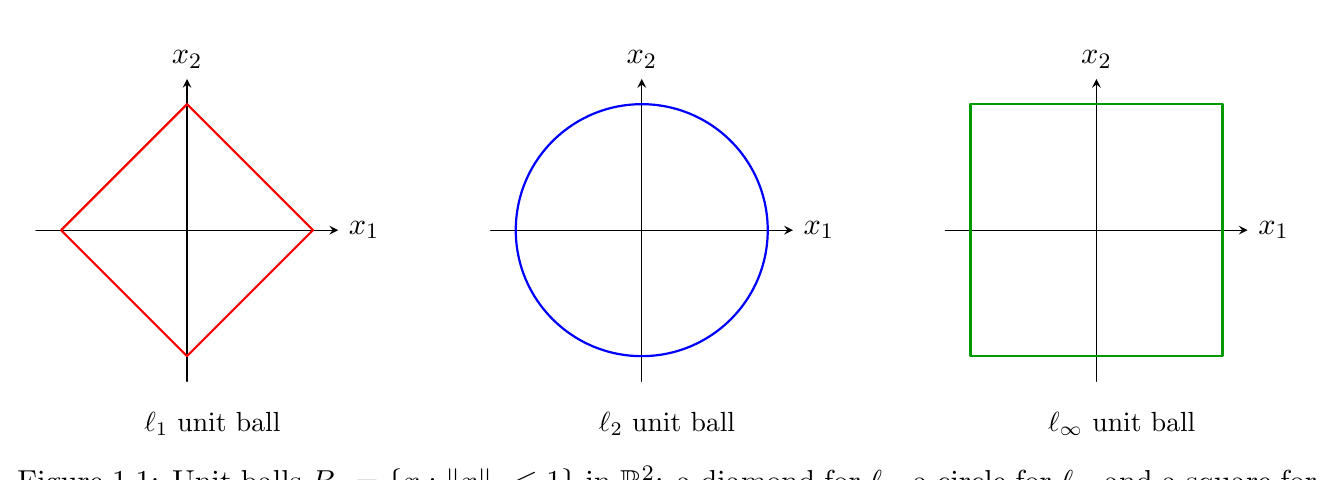
\includegraphics[width=0.8\linewidth]{unit_balls}}
\figcap{Figure 1.1 of the notes: the unit balls $B_p=\{x:\norm x_p\le1\}$ in $\R^2$, a diamond for $\ell_1$, a circle for $\ell_2$, a square for $\ell_\infty$.
They are nested, $B_1\subseteq B_2\subseteq B_\infty$, which is the picture behind $\norm x_\infty\le\norm x_2\le\norm x_1$.}
\end{center}

\begin{defn}[The ``$\ell_0$ norm'']
$\norm x_0$ = the \term{number of nonzero entries} of $x$. Example: $\norm{(3,0,0,-1)}_0 = 2$. It is the natural measure of
\term{sparsity} and returns in Chapter 13.
\end{defn}

\begin{pitfall}[$\ell_0$ is not a norm]
It fails homogeneity: $\norm{2x}_0 = \norm x_0$, not $2\norm x_0$. For $x=(1,0)$: $\norm{2x}_0 = 1 \neq 2 = 2\norm x_0$.
\end{pitfall}

\subsection{All norms are equivalent}

\begin{formula}[Equivalence of norms]
On $\R^n$ every two norms are related by constant factors that do not depend on $x$. For our three norms (proved in Exercise 1.3):
\[ \norm x_\infty \le \norm x_2 \le \sqrt n\,\norm x_\infty,\qquad \norm x_2\le\norm x_1\le\sqrt n\,\norm x_2. \]
\end{formula}

\begin{intuition}[Why this matters]
If an algorithm makes the error small in one norm, it is small in every norm. The constants can depend on the dimension $n$, though, so in
high dimension the choice of norm does matter quantitatively.
\end{intuition}

\subsection{The Cauchy--Schwarz inequality}

\begin{formula}[Theorem 1.2: Cauchy--Schwarz]
For all $a,b\in\R^n$:\qquad $|a^Tb|\le\norm a_2\,\norm b_2$,\qquad with equality if and only if $a$ and $b$ are linearly dependent.
\end{formula}

\textbf{Proof, step by step} (the lecture's proof uses an optimization problem):
\begin{enumerate}
  \item If $b=0$ both sides are $0$. Assume $b\ne 0$.
  \item For any scalar $c$, a norm squared is never negative: $0\le\norm{a-cb}_2^2$. So also $0\le\min_c\norm{a-cb}_2^2$.
  \item Expand: $\norm{a-cb}_2^2 = (a-cb)^T(a-cb) = \norm a^2 - 2c\,a^Tb + c^2\norm b^2$. This is a parabola in $c$.
  \item Minimize: set the derivative $-2a^Tb + 2c\norm b^2$ to $0$, giving $c_{\text{opt}} = \dfrac{a^Tb}{b^Tb}$.
  \item Plug in: $\norm a^2 - 2\dfrac{(a^Tb)^2}{\norm b^2} + \dfrac{(a^Tb)^2}{\norm b^2} = \norm a^2 - \dfrac{(a^Tb)^2}{\norm b^2}$. So
        \[ 0\le\norm a_2^2 - \frac{(a^Tb)^2}{\norm b_2^2}\quad\Longrightarrow\quad (a^Tb)^2\le\norm a_2^2\norm b_2^2. \]
  \item Take square roots. Equality holds exactly when $\min_c\norm{a-cb}=0$, i.e.\ $a=cb$ for some $c$: $a$ and $b$ are linearly dependent.
\end{enumerate}

\begin{center}
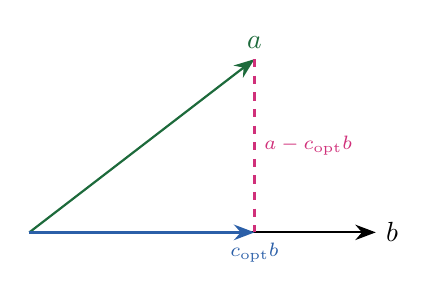
\begin{tikzpicture}[scale=1.1]
  \draw[->,thick] (0,0)--(4,0) node[right]{$b$};
  \draw[->,thick,pgreen] (0,0)--(2.6,2) node[above]{$a$};
  \draw[dashed,ppink,thick] (2.6,2)--(2.6,0);
  \draw[->,very thick,pcyan] (0,0)--(2.6,0) node[below,font=\scriptsize]{$c_{\text{opt}}b$};
  \node[ppink,font=\scriptsize,right] at (2.6,1){$a-c_{\text{opt}}b$};
\end{tikzpicture}
\figcap{$c_{\text{opt}}b$ is the projection of $a$ on the line of $b$. The leftover $a-c_{\text{opt}}b$ has length $\ge0$; that is the whole proof.}
\end{center}

\begin{example}[Checking it]
$a=(1,2)$, $b=(3,1)$: $|a^Tb| = 3+2 = 5$, and $\norm a\norm b = \sqrt5\sqrt{10} = \sqrt{50}\approx 7.07$. Indeed $5\le7.07$.
With $a=(2,4)=2\cdot(1,2)$ and $b=(1,2)$: $a^Tb = 10 = \sqrt{20}\sqrt5$, equality, since $a$ is a multiple of $b$.
\end{example}

\section{Matrices}

We mostly distinguish \hl{square symmetric matrices} from rectangular ones.

\begin{defn}[Basic notions]
\begin{itemize}
  \item \term{Trace}: $\Tr\{A\} = \sum_iA_{ii}$ for square $A$ (sum of the diagonal). It is \term{cyclic}: $\Tr\{AB\} = \Tr\{BA\}$.
  \item \term{Diagonals}: $\diag(A)$ extracts the diagonal of a matrix as a vector; $\Diag(a)$ builds a diagonal matrix from a vector.
  \item \term{Determinant}: $\det(A)$.
\end{itemize}
Example: $A=\begin{pmatrix}1&2\\3&4\end{pmatrix}$: $\Tr A=5$, $\diag(A)=(1,4)$, $\Diag(1,4)=\begin{pmatrix}1&0\\0&4\end{pmatrix}$, $\det A = 4-6=-2$.
\end{defn}

\begin{pitfall}[Cyclic, not commutative]
$\Tr\{AB\}=\Tr\{BA\}$ even though $AB\neq BA$ in general. For three matrices you may \emph{rotate}, $\Tr\{ABC\}=\Tr\{CAB\}=\Tr\{BCA\}$,
but not swap: $\Tr\{ABC\}\neq\Tr\{BAC\}$ in general.
\end{pitfall}

\subsection{Eigenvalues (briefly)}

\begin{defn}[Eigenpair]
An \term{eigenpair} of a square matrix $A$ is a scalar $\lambda$ and a vector $v\ne0$ with $Av=\lambda v$.
\end{defn}

\textbf{How to find eigenvalues.} Rewrite $Av=\lambda v$ as $(A-\lambda I)v=0$. A nonzero solution $v$ exists exactly when
$A-\lambda I$ is singular:
\[ \det(A-\lambda I)=0. \]

\begin{defn}[Diagonalizable]
$A$ is \term{diagonalizable} if it is similar to a diagonal matrix: $A = U\Diag\{\lambda_i\}U^{-1}$, with the eigenvectors as the columns of $U$.
\end{defn}

\begin{example}[Not every matrix is diagonalizable: $A=\begin{pmatrix}0&1\\0&0\end{pmatrix}$]
\begin{enumerate}
  \item $\det(A-\lambda I)=\lambda^2$, so the only eigenvalue is $\lambda=0$ (twice).
  \item If $A = U\Diag(0,0)U^{-1}$, then $A = U\cdot 0\cdot U^{-1} = 0$. But $A\neq0$. Contradiction.
\end{enumerate}
(The eigenvectors are only the multiples of $(1,0)$: there are not enough of them to build an invertible $U$.)
\end{example}

\begin{formula}[Theorem 1.3: Spectral theorem]
Every \textbf{real symmetric} matrix has \textbf{real} eigenvalues and is diagonalizable by an \textbf{orthogonal} matrix:
\[ A = U\Diag\{\lambda_i\}U^T,\qquad U^TU=UU^T=I. \]
\end{formula}

\begin{intuition}[Why symmetric matrices are so pleasant]
For a symmetric matrix, $U^{-1}$ is just $U^T$, and the eigenvectors are perpendicular. So \hl{a symmetric matrix only stretches space
along perpendicular axes}: by $\lambda_1$ along $u_1$, by $\lambda_2$ along $u_2$, and so on.
\end{intuition}

\subsection{The $2\times2$ symmetric case}

For $A = \begin{pmatrix}a&c\\c&b\end{pmatrix}$:
\[ \det\begin{pmatrix}a-\lambda&c\\c&b-\lambda\end{pmatrix} = (a-\lambda)(b-\lambda)-c^2 = \lambda^2-(a+b)\lambda+(ab-c^2)=0, \]
\[ \lambda_{1,2} = \frac{a+b\pm\sqrt{(a+b)^2-4(ab-c^2)}}{2}. \]

\begin{formula}[Trace and determinant in terms of eigenvalues]
For symmetric $A$ (using cyclicity and $U^TU=I$):
\[ \Tr\{A\} = \Tr\{U\Diag\{\lambda_i\}U^T\} = \Tr\{U^TU\Diag\{\lambda_i\}\} = \sum_i\lambda_i,\qquad \det(A)=\prod_i\lambda_i. \]
\end{formula}

\begin{example}[$A=\begin{pmatrix}2&1\\1&2\end{pmatrix}$]
$a=b=2$, $c=1$: $\lambda^2-4\lambda+3=0$, so $\lambda\in\{3,1\}$.
Eigenvectors: $(A-3I)v=0\Rightarrow v\propto(1,1)$; $(A-I)v=0\Rightarrow v\propto(1,-1)$. Normalized:
\[ U=\tfrac1{\sqrt2}\begin{pmatrix}1&1\\1&-1\end{pmatrix},\qquad A = U\Diag(3,1)U^T. \]
Check: $\Tr A = 4 = 3+1$ and $\det A = 4-1 = 3 = 3\cdot1$. The two eigenvectors are perpendicular: $(1,1)\cdot(1,-1)=0$.
\end{example}

\section{Positive definiteness}

Positive definiteness is the matrix version of ``$x>0$''. It is the most important matrix property in this course.

\begin{defn}[Definition 1.4: PD and PSD]
A \textbf{symmetric} matrix $X$ is
\begin{itemize}
  \item \term{positive definite}, written $X\succ0$, if $z^TXz>0$ for all $z\ne0$;
  \item \term{positive semidefinite}, written $X\succeq0$, if $z^TXz\ge0$ for all $z$.
\end{itemize}
For symmetric $A,B$ we write $A\succ B$ to mean $A-B\succ0$ (and $A\succeq B$ for $A-B\succeq0$), just as with numbers.
\end{defn}

\begin{example}[Computing $z^TXz$]
$X=\begin{pmatrix}2&1\\1&2\end{pmatrix}$, $z=(z_1,z_2)$:
$z^TXz = 2z_1^2+2z_1z_2+2z_2^2 = z_1^2+z_2^2+(z_1+z_2)^2$. A sum of squares, and it is $0$ only if $z_1=z_2=0$. So $X\succ0$.

$Y=\begin{pmatrix}1&2\\2&1\end{pmatrix}$, $z=(1,-1)$: $z^TYz = 1-4+1 = -2<0$. So $Y$ is \emph{not} PSD, even though all its entries are positive.
\end{example}

\begin{pitfall}[Positive entries $\neq$ positive definite]
$Y$ above has all entries positive and is not PSD. Conversely $\begin{pmatrix}2&-1\\-1&2\end{pmatrix}\succ0$ has negative entries.
PD is about $z^TXz$, not about the signs of the entries. Throughout the course, positivity statements always refer to \textbf{symmetric} matrices.
\end{pitfall}

\begin{intuition}[Only a partial order]
For numbers, either $a\ge b$ or $b\ge a$. For matrices this fails: \hl{two matrices may be incomparable}.
Example: $A=\Diag(2,1)$, $B=\Diag(1,2)$. Then $A-B=\Diag(1,-1)$ is neither $\succeq0$ nor $\preceq0$
($z=(1,0)$ gives $+1$, $z=(0,1)$ gives $-1$). So neither $A\succeq B$ nor $B\succeq A$.
\end{intuition}

\subsection{Two equivalent tests for $X\succ0$}

\begin{formula}[Test 1: Cholesky]
$X\succ0$ \textbf{if and only if} $X=LL^T$ with $L$ lower triangular with positive diagonal (the \term{Cholesky decomposition},
the matrix version of a square root). This is the standard \emph{numerical} test for positive definiteness. For $2\times2$:
\[ \begin{pmatrix}a&c\\c&b\end{pmatrix} = \begin{pmatrix}\sqrt a&0\\ \frac{c}{\sqrt a}&\sqrt{b-\frac{c^2}{a}}\end{pmatrix}
\begin{pmatrix}\sqrt a&\frac{c}{\sqrt a}\\ 0&\sqrt{b-\frac{c^2}{a}}\end{pmatrix},\qquad a>0,\ \ ab-c^2>0. \]
\end{formula}

\textbf{Why exactly those two conditions?} The square roots must be of positive numbers: $a>0$ for $\sqrt a$, and $b-c^2/a>0$,
i.e.\ (multiplying by $a>0$) $ab-c^2>0$. If either fails, there is no real $L$ with a positive diagonal.

\begin{example}[$2\times2$ Cholesky]
$A=\begin{pmatrix}4&2\\2&3\end{pmatrix}$: $a=4$, $c=2$, $b=3$.
$L_{11}=\sqrt4=2$, $L_{21}=2/2=1$, $L_{22}=\sqrt{3-4/4}=\sqrt2$.
\[ L=\begin{pmatrix}2&0\\1&\sqrt2\end{pmatrix},\qquad LL^T = \begin{pmatrix}4&2\\2&1+2\end{pmatrix} = A.\ \checkmark \]
\end{example}

The construction generalizes recursively via the \emph{Schur complement} (Chapter 8).

\begin{formula}[Test 2: eigenvalues]
$X\succ0$ \textbf{if and only if} all eigenvalues of $X$ are positive. ($X\succeq0$ iff all are $\ge0$.)
\end{formula}

\textbf{Proof.}
\begin{itemize}
  \item[($\Rightarrow$)] If $X = UDU^T\succ0$, choose $z=u_j$ (the $j$-th eigenvector, a unit vector). Then $u_j^TXu_j = u_j^T(\lambda_ju_j) = \lambda_j>0$.
  \item[($\Leftarrow$)] If all $\lambda_i>0$, then for any $z\ne0$, set $w=U^Tz\ne0$ ($U^T$ is invertible):
        \[ z^TXz = z^TUDU^Tz = w^TDw = \sum_i\lambda_i\,w_i^2 = \sum_i\lambda_i[U^Tz]_i^2>0. \]
\end{itemize}

\begin{formula}[$2\times2$ shortcut]
Both eigenvalues of $\begin{pmatrix}a&c\\c&b\end{pmatrix}$ are positive $\iff$ trace and determinant are positive:
\[ a+b>0\ \text{ and }\ ab-c^2>0\qquad\Longleftrightarrow\qquad a>0\ \text{ and }\ ab-c^2>0. \]
\end{formula}

\textbf{Why the two versions agree.} If $ab-c^2>0$ then $ab>c^2\ge0$, so $a$ and $b$ have the same sign. Then $a+b>0$ and $a>0$ say the same thing.

\begin{example}[Three quick checks]
\begin{center}
\renewcommand{\arraystretch}{1.3}
\begin{tabular}{>{\columncolor{border}}c c c l}
\thd{$X$} & \cellcolor{border}\thd{$a$} & \cellcolor{border}\thd{$ab-c^2$} & \cellcolor{border}\thd{VERDICT}\\
\rowcolor{surface} \cellcolor{border}\color{surface}$\begin{pmatrix}2&1\\1&2\end{pmatrix}$ & $2$ & $3$ & $\succ0$ (eigenvalues 3, 1)\\
\rowcolor{surface2} \cellcolor{border}\color{surface}$\begin{pmatrix}1&2\\2&1\end{pmatrix}$ & $1$ & $-3$ & not PSD (eigenvalues 3, $-1$)\\
\rowcolor{surface} \cellcolor{border}\color{surface}$\begin{pmatrix}1&1\\1&1\end{pmatrix}$ & $1$ & $0$ & $\succeq0$ but not $\succ0$ (eigenvalues 2, 0)\\
\end{tabular}
\end{center}
\end{example}

\begin{plainbox}
\textbf{Food for thought (from the lecture).} Does $A\succ B\succ0$ imply $B^{-1}\succ A^{-1}$? For numbers: $3>2>0$ gives $\frac12>\frac13$.
The matrix answer is \textbf{yes}; it is proved in the recitation, Exercise 1.8(2).
\end{plainbox}

\section{Matrix norms}

Matrices also have norms, but the terminology is less standard and can be confusing. Two matter here.

\begin{defn}[Frobenius norm]
$\norm A_{\mathrm{Fro}} = \sqrt{\sum_{ij}A_{ij}^2}$: treat $A$ as one long vector and take its $\ell_2$ norm.
\end{defn}

\begin{defn}[Spectral norm]
$\norm A_2 = \max_{x:\,\norm x_2=1}\norm{Ax}_2$: \hl{the largest factor by which $A$ can stretch a vector}.
\end{defn}

\begin{intuition}[In terms of singular values (Chapter 3)]
The Frobenius norm is the $\ell_2$ norm of the singular values; the spectral norm is their maximum. For a symmetric matrix the singular
values are $|\lambda_i|$, so $\norm A_2 = \max_i|\lambda_i|$.
\end{intuition}

\begin{example}[Both norms of $A=\begin{pmatrix}2&1\\1&2\end{pmatrix}$]
$\norm A_{\mathrm{Fro}}=\sqrt{4+1+1+4}=\sqrt{10}\approx3.16$, and indeed $\sqrt{3^2+1^2}=\sqrt{10}$.
$\norm A_2 = \max(3,1) = 3$, attained at $x=\frac1{\sqrt2}(1,1)$: $Ax = \frac1{\sqrt2}(3,3)$, of length $3$.
Always $\norm A_2\le\norm A_{\mathrm{Fro}}$ (a maximum is at most the root of the sum of squares).
\end{example}

\begin{pitfall}[$\norm A_2$ is not the $\ell_2$ norm of the entries]
For a matrix, ``$\norm A_2$'' means the \emph{spectral} norm. The $\ell_2$ norm of the entries is the Frobenius norm.
\end{pitfall}

\section{Linear systems}

The core computational problem of linear algebra is solving $Ax=b$. There are three possible cases:
\begin{itemize}
  \item a \textbf{unique solution}, typically when $A$ is square and invertible: $x=A^{-1}b$;
  \item \textbf{no solution};
  \item \textbf{infinitely many solutions}.
\end{itemize}

\begin{example}[One of each]
$\begin{pmatrix}1&1\\1&-1\end{pmatrix}x=\begin{pmatrix}2\\0\end{pmatrix}$: unique, $x=(1,1)$.\quad
$\begin{pmatrix}1&1\\1&1\end{pmatrix}x=\begin{pmatrix}2\\3\end{pmatrix}$: none ($x_1+x_2$ cannot be both $2$ and $3$).\quad
$\begin{pmatrix}1&1\\1&1\end{pmatrix}x=\begin{pmatrix}2\\2\end{pmatrix}$: infinitely many ($x=(t,2-t)$).
\end{example}

\begin{intuition}[A fourth, in-between regime]
In practice there is a fourth case: $A$ is invertible but only \emph{barely} (\term{ill-conditioned}). Then a tiny change in $b$ can change $x$ enormously.
This is quantified by the condition number in the recitation (Exercise 1.4).
\end{intuition}

\subsection{How do we solve linear systems numerically?}

\begin{itemize}
  \item \textbf{Direct (non-iterative) methods}: now and in the recitation. They give the exact answer (up to rounding) in a fixed number of steps.
  \item \textbf{Iterative methods}: in a few weeks.
\end{itemize}
The two classical direct methods are the \term{LU} decomposition (general square matrices, Part C) and the \term{Cholesky} decomposition
(positive definite matrices, below). Both solve systems in a numerically stable and efficient way.

\begin{pitfall}[Don't compute $A^{-1}$]
$x=A^{-1}b$ is the right formula on paper, but numerically we never form $A^{-1}$. It costs more and is less stable.
We factor $A$ into triangular pieces and solve triangular systems instead \src{BV C.2}.
\end{pitfall}

\section{Solving with Cholesky}

If $A\in\R^{n\times n}$ is symmetric positive definite, it has a Cholesky decomposition $A=LL^T$, where $L$ is the \emph{unique}
lower triangular matrix with positive diagonal.

\begin{formula}[Computing $L$ (Golub \& Van Loan, Alg.\ 4.2.1)]
\begin{tabular}{@{}l@{}}
Initialize $L$ as an $n\times n$ zero matrix.\\
\textbf{for} $j=1,\dots,n$:\\
\quad $v_{j:n} = A_{j:n,\,j}$ \hfill(the part of column $j$ on and below the diagonal)\\
\quad \textbf{for} $k=1,\dots,j-1$:\quad $v_{j:n} = v_{j:n} - L_{j,k}\,L_{j:n,\,k}$ \hfill(remove earlier columns)\\
\quad $L_{j:n,\,j} = v_{j:n}/\sqrt{v_j}$ \hfill(normalize by the root of the new pivot)\\
After the loop, $L$ is lower triangular and $A=LL^T$.
\end{tabular}
\end{formula}

\begin{formula}[Solving $Ax=b$]
\begin{enumerate}
  \item Compute $L$ with $A=LL^T$.
  \item Solve $Ly=b$ by \term{forward substitution} (top row first).
  \item Solve $L^Tx=y$ by \term{backward substitution} (bottom row first).
\end{enumerate}
Why it works: $Ax = L(L^Tx) = Ly = b$.
\end{formula}

\begin{example}[A full $3\times3$ solve]
$A=\begin{pmatrix}4&2&2\\2&5&3\\2&3&6\end{pmatrix}$, $b=(10,13,17)$.

\textbf{Factor.}
\begin{itemize}
  \item $j=1$: $v=(4,2,2)$, $L_{:,1}=v/\sqrt4=(2,1,1)$.
  \item $j=2$: $v_{2:3}=(5,3)-L_{21}\,L_{2:3,1}=(5,3)-1\cdot(1,1)=(4,2)$; $L_{2:3,2}=(4,2)/\sqrt4=(2,1)$.
  \item $j=3$: $v_3=6-L_{31}L_{31}-L_{32}L_{32}=6-1-1=4$; $L_{33}=\sqrt4=2$.
\end{itemize}
$L=\begin{pmatrix}2&0&0\\1&2&0\\1&1&2\end{pmatrix}$. All pivots were positive, which also certifies $A\succ0$.

\textbf{Forward} $Ly=b$: $y_1=10/2=5$, $y_2=(13-1\cdot5)/2=4$, $y_3=(17-5-4)/2=4$.

\textbf{Backward} $L^Tx=y$ with $L^T=\begin{pmatrix}2&1&1\\0&2&1\\0&0&2\end{pmatrix}$: $x_3=4/2=2$, $x_2=(4-2)/2=1$, $x_1=(5-1-2)/2=1$.

$x=(1,1,2)$. Check: $Ax=(4+2+4,\ 2+5+6,\ 2+3+12)=(10,13,17)=b$. \checkmark
\end{example}

\begin{formula}[Complexity]
Cholesky factorization $\approx\frac13n^3$ flops; each triangular solve $O(n^2)$; total $O(n^3)$, but with \hl{half the constant of LU} ($\approx\frac23n^3$).
\end{formula}

\begin{example}[What the constants mean]
For $n=1000$: Cholesky $\approx3.3\times10^8$ flops, LU $\approx6.7\times10^8$, one triangular solve $\approx10^6$.
The factorization dominates. Once it is done, every new right-hand side $b$ is cheap.
\end{example}

% =================================================================
\parttitle{PART B \textperiodcentered\ RECITATION 1}{Exercises: Norms, Conditioning, PSD Matrices}
% =================================================================

\section{Exercise 1.1: three norms of three vectors}

\begin{example}[Exercise 1.1 \ $\bullet\circ\circ$]
Compute $\norm x_1,\norm x_2,\norm x_\infty$ for $x=(1,0,0,0)$, $(1,1,1,1)$, $(3,-1,2,0)$ and verify $\norm x_\infty\le\norm x_2\le\norm x_1$.
Which vectors make which inequalities tight?
\end{example}

\textbf{Solution.}
\begin{center}
\renewcommand{\arraystretch}{1.3}
\begin{tabular}{>{\columncolor{border}}c c c c l}
\thd{$x$} & \cellcolor{border}\thd{$\norm x_1$} & \cellcolor{border}\thd{$\norm x_2$} & \cellcolor{border}\thd{$\norm x_\infty$} & \cellcolor{border}\thd{COMMENT}\\
\rowcolor{surface} \cellcolor{border}\color{surface}$(1,0,0,0)$ & 1 & 1 & 1 & 1-sparse: all norms coincide\\
\rowcolor{surface2} \cellcolor{border}\color{surface}$(1,1,1,1)$ & 4 & $\sqrt4=2$ & 1 & flat: as far apart as possible\\
\rowcolor{surface} \cellcolor{border}\color{surface}$(3,-1,2,0)$ & $3+1+2=6$ & $\sqrt{14}\approx3.74$ & 3 & $3<3.74<6$ (strict)\\
\end{tabular}
\end{center}

\begin{intuition}[Sparse vs.\ flat]
\hl{A vector with a single nonzero entry collapses all three norms to the same value. A flat vector spreads them as far apart as possible.}
For $(1,1,1,1)$: $\norm x_2 = 2 = \sqrt4\cdot\norm x_\infty$ and $\norm x_1 = 4 = \sqrt4\cdot\norm x_2$, so the upper constants of Exercise 1.3 are attained.
\end{intuition}

\section{Exercise 1.2: $\ell_2$ is a norm}

\begin{example}[Exercise 1.2 \ $\bullet\circ\circ$]
Using only the properties of the inner product and Cauchy--Schwarz, verify that $f(x)=\sqrt{x^Tx}$ satisfies the three norm axioms.
\end{example}

\textbf{Solution.}
\begin{enumerate}
  \item \textbf{Positive definiteness.} $x^Tx=\sum_ix_i^2\ge0$ (a sum of squares), and it is $0$ iff every $x_i=0$. The square root keeps both facts.
  \item \textbf{Homogeneity.} $\sqrt{(\alpha x)^T(\alpha x)} = \sqrt{\alpha^2\,x^Tx} = \sqrt{\alpha^2}\sqrt{x^Tx} = |\alpha|\sqrt{x^Tx}$.
  \item \textbf{Triangle inequality.} Expand the square, then use Cauchy--Schwarz on the middle term ($x^Ty\le\norm x_2\norm y_2$):
  \[ \norm{x+y}_2^2 = x^Tx+2x^Ty+y^Ty \le \norm x_2^2+2\norm x_2\norm y_2+\norm y_2^2 = (\norm x_2+\norm y_2)^2. \]
  Both sides are nonnegative, so take square roots.
\end{enumerate}

\begin{pitfall}[Logical order]
Cauchy--Schwarz was proved directly (lecture), and the triangle inequality \emph{follows} from it, not the other way around. Using the
triangle inequality for $\ell_2$ inside this proof would be circular.
\end{pitfall}

\begin{pitfall}[$\sqrt{\alpha^2}=|\alpha|$]
Not $\alpha$. With $\alpha=-2$: $\sqrt{4}=2=|-2|$. This is where the absolute value in the homogeneity axiom comes from.
\end{pitfall}

\section{Exercise 1.3: sharp equivalence constants}

\begin{example}[Exercise 1.3 \ $\bullet\bullet\circ$]
Prove for all $x\in\R^n$:\quad $\norm x_2\le\norm x_1\le\sqrt n\,\norm x_2$\quad and\quad $\norm x_\infty\le\norm x_2\le\sqrt n\,\norm x_\infty$,
and exhibit vectors attaining each inequality with equality.
\end{example}

\textbf{Solution, one inequality at a time.}
\begin{enumerate}
  \item $\norm x_\infty\le\norm x_2$: for every $i$, $x_i^2\le\sum_jx_j^2$, so $|x_i|\le\norm x_2$. Take the max over $i$.
  \item $\norm x_2\le\sqrt n\norm x_\infty$: replace every entry by the largest one,
        $\norm x_2^2=\sum_ix_i^2\le\sum_i\big(\max_j|x_j|\big)^2 = n\norm x_\infty^2$. Take square roots.
  \item $\norm x_2\le\norm x_1$: $\big(\sum_i|x_i|\big)^2 = \sum_ix_i^2 + \sum_{i\ne j}|x_i||x_j| \ge \sum_ix_i^2$ (the cross terms are $\ge0$). Take square roots.
  \item $\norm x_1\le\sqrt n\norm x_2$: Cauchy--Schwarz with the all-ones vector $\mathbf 1$ and $|x|=(|x_1|,\dots,|x_n|)$:
        \[ \norm x_1 = \mathbf 1^T|x| \le \norm{\mathbf 1}_2\,\norm{|x|}_2 = \sqrt n\,\norm x_2. \]
\end{enumerate}

\textbf{Tightness.} The left inequalities are equalities for 1-sparse vectors such as $(1,0,\dots,0)$ (all norms equal $1$).
The right ones are equalities for flat vectors such as $\mathbf 1=(1,\dots,1)$: $\norm{\mathbf 1}_2=\sqrt n=\sqrt n\norm{\mathbf 1}_\infty$
and $\norm{\mathbf1}_1 = n = \sqrt n\cdot\sqrt n$ (equality in Cauchy--Schwarz, since $|x|$ is a multiple of $\mathbf 1$).

\section{Exercise 1.4: the condition number}

\begin{defn}[Condition number]
For invertible $A\in\R^{n\times n}$: $\kappa(A)=\norm A_2\cdot\norm{A^{-1}}_2$. For symmetric $A$ this is $\dfrac{\max_i|\lambda_i|}{\min_i|\lambda_i|}$.
Always $\kappa(A)\ge1$.
\end{defn}

\begin{example}[Exercise 1.4 \ $\bullet\bullet\circ$]
(1) Prove: if $Ax=b$ and $A\tilde x=b+\delta b$, then $\dfrac{\norm{\tilde x-x}_2}{\norm x_2}\le\kappa(A)\cdot\dfrac{\norm{\delta b}_2}{\norm b_2}$.\\
(2) Demonstrate it on $A=\begin{pmatrix}1&0.99\\0.99&0.98\end{pmatrix}$, $b=\begin{pmatrix}0.99\\0.98\end{pmatrix}$, $\tilde b=\begin{pmatrix}0.99\\0.981\end{pmatrix}$.
\end{example}

\textbf{The tool used twice:} $\norm{Mv}_2\le\norm M_2\norm v_2$. It follows from the definition of the spectral norm:
for $v\ne0$, $u=v/\norm v$ is a unit vector, and a maximum is at least each of its values, so $\norm{Mv}/\norm v = \norm{Mu}\le\norm M_2$.

\textbf{Solution (1).}
\begin{enumerate}
  \item Subtract the two systems: $A\tilde x - Ax = \delta b$, i.e.\ $A(\tilde x-x)=\delta b$, so $\tilde x-x = A^{-1}\delta b$.
  \item Apply the tool with $M=A^{-1}$: $\;\norm{\tilde x-x}_2 = \norm{A^{-1}\delta b}_2 \le \norm{A^{-1}}_2\,\norm{\delta b}_2$.
  \item Apply it with $M=A$, $v=x$: $\;\norm b_2 = \norm{Ax}_2\le\norm A_2\norm x_2$, hence $\dfrac1{\norm x_2}\le\dfrac{\norm A_2}{\norm b_2}$ (assume $b\ne0$).
  \item Multiply the inequalities of steps 2 and 3 (all terms nonnegative):
        \[ \frac{\norm{\tilde x-x}_2}{\norm x_2}\le\underbrace{\norm A_2\norm{A^{-1}}_2}_{\kappa(A)}\frac{\norm{\delta b}_2}{\norm b_2}. \]
\end{enumerate}

\textbf{Solution (2), with numbers.}
\begin{enumerate}
  \item $\det A = 1\cdot0.98-0.99^2 = 0.98-0.9801 = -10^{-4}$: invertible, but barely.
  \item Eigenvalues ($\Tr=1.98$, $\det=-10^{-4}$): $\lambda=\frac{1.98\pm\sqrt{1.98^2+4\cdot10^{-4}}}{2}$, so
        $\lambda_1\approx1.98$, $\lambda_2\approx-5.05\cdot10^{-5}$. $A$ is symmetric, so $\kappa(A) = |\lambda_1|/|\lambda_2|\approx\hl{3.9\cdot10^4}$.
  \item Solve $Ax=b$: $b$ is exactly the second column of $A$, so $x=(0,1)$.
  \item Solve $A\tilde x=\tilde b$ (Cramer's rule):
        $\tilde x_1 = \frac{0.99\cdot0.98-0.99\cdot0.981}{-10^{-4}} = \frac{-0.00099}{-10^{-4}} = 9.9$,\quad
        $\tilde x_2 = \frac{1\cdot0.981-0.99\cdot0.99}{-10^{-4}} = \frac{0.0009}{-10^{-4}} = -9$.\\
        Check: $9.9-0.99\cdot9 = 0.99$ and $0.99\cdot9.9-0.98\cdot9 = 9.801-8.82 = 0.981$. \checkmark
  \item Relative changes: $\dfrac{\norm{\tilde x-x}}{\norm x} = \norm{(9.9,-10)} = \sqrt{198.01}\approx14.1$, while
        $\dfrac{\norm{\tilde b-b}}{\norm b} = \dfrac{0.001}{\sqrt{0.9801+0.9604}}\approx7.2\cdot10^{-4}$.
  \item Amplification $\approx14.1/(7.2\cdot10^{-4})\approx\hl{2\cdot10^4}\le\kappa\approx3.9\cdot10^4$. Same order, consistent with the bound.
\end{enumerate}

\begin{center}
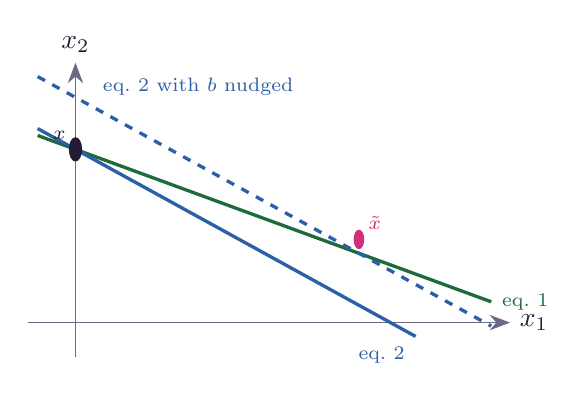
\begin{tikzpicture}[xscale=1.2,yscale=2.2]
  \draw[->,muted] (-0.5,0)--(4.6,0) node[right,ink]{$x_1$};
  \draw[->,muted] (0,-0.2)--(0,1.5) node[above,ink]{$x_2$};
  \draw[pgreen,very thick] (-0.4,1.08)--(4.4,0.12) node[right,font=\scriptsize]{eq.\ 1};
  \draw[pcyan,very thick] (-0.4,1.12)--(3.6,-0.08) node[below left,font=\scriptsize]{eq.\ 2};
  \draw[pcyan,very thick,dashed] (-0.4,1.42)--(4.4,-0.02) node[pos=0.12,above right,font=\scriptsize]{eq.\ 2 with $b$ nudged};
  \fill[ink] (0,1) circle (2pt) node[above left,font=\scriptsize]{$x$};
  \fill[ppink] (3,0.48) circle (1.6pt) node[above right,font=\scriptsize]{$\tilde x$};
\end{tikzpicture}
\figcap{Schematic: the two equations of an ill-conditioned system are almost parallel lines. Moving one line a tiny bit slides
their crossing point far along them. That is why $\tilde x$ is so far from $x$.}
\end{center}

\begin{intuition}[Morals]
\begin{itemize}
  \item $\kappa(A)\approx1$: well-conditioned. $\kappa(A)\gg1$: small errors in $b$ (or rounding errors) may cause large errors in $x$.
  \item The condition number is a property of the \hl{matrix}, not of the algorithm. No clever solver can undo it.
\end{itemize}
\end{intuition}

\section{Exercise 1.5: the matrix inner product}

\begin{example}[Exercise 1.5 \ $\bullet\circ\circ$]
For $A,B\in\R^{m\times n}$ define $\langle A,B\rangle=\Tr\{B^TA\}$.
(1) Show it is an inner product on $\R^{m\times n}$. Deduce (2) $\norm A_{\mathrm{Fro}}^2=\Tr\{AA^T\}$, (3) $\Tr\{AB^T\}=\Tr\{A^TB\}$,
(4) $\Tr\{xy^T\}=x^Ty$ for vectors $x,y$.
\end{example}

\textbf{Solution.}
\begin{enumerate}
  \item Write it with indices: $(B^TA)_{jj} = \sum_iB_{ij}A_{ij}$, so $\Tr\{B^TA\} = \sum_{ij}A_{ij}B_{ij}$.
        Stack the entries of each matrix into a long vector in $\R^{mn}$: this is exactly the standard inner product there.
        So symmetry, linearity and positive definiteness hold because they hold in $\R^{mn}$.
  \item Take $B=A$: $\langle A,A\rangle = \sum_{ij}A_{ij}^2 = \norm A_{\mathrm{Fro}}^2$ (the Frobenius norm is the norm induced by this inner product).
        By cyclicity, $\Tr\{A^TA\}=\Tr\{AA^T\}$.
  \item Both sides equal $\sum_{ij}A_{ij}B_{ij}$.
  \item A special case of (3) with $m\times1$ matrices, or directly: $\Tr\{xy^T\} = \Tr\{y^Tx\} = y^Tx = x^Ty$, since the trace of a scalar is itself.
        This little identity is used constantly from Chapter 9 on.
\end{enumerate}

\begin{example}[Numbers]
$A=\begin{pmatrix}1&2\\3&4\end{pmatrix}$, $B=\begin{pmatrix}0&1\\1&0\end{pmatrix}$: $\langle A,B\rangle = 1\cdot0+2\cdot1+3\cdot1+4\cdot0 = 5$.
Via the trace: $B^TA = \begin{pmatrix}3&4\\1&2\end{pmatrix}$, trace $3+2=5$. \checkmark
\end{example}

\section{Exercise 1.6: entries of a PSD matrix}

\begin{defn}[The three matrix sets]
\[ S^d=\{A\in\R^{d\times d}:A=A^T\},\qquad S^d_+=\{A\in S^d:A\succeq0\},\qquad S^d_{++}=\{A\in S^d:A\succ0\}. \]
Symmetric, positive semidefinite, and positive definite matrices.
\end{defn}

\begin{example}[Exercise 1.6 \ $\bullet\circ\circ$]
Let $A\in S^d_+$. Prove: (1) $A_{ii}\ge0$ for every $i$; (2) $\det(A)\ge0$; (3) the maximal entry of $A$ is on the diagonal,
$\max_{l,k}A_{lk}=\max_iA_{ii}$; (4) if $A_{ii}=0$ for some $i$, then $A_{ij}=0$ for every $j$.
\end{example}

\textbf{Solution.} The trick throughout: \hl{choose a clever test vector $z$ and use $z^TAz\ge0$}.
\begin{enumerate}
  \item With the standard basis vector $z=e_i$: $A_{ii} = e_i^TAe_i\ge0$.
  \item By the spectral theorem $A=U\Sigma U^T$, so
        $\det(A) = \det(U)\det(\Sigma)\det(U^T) = \det(UU^T)\det(\Sigma) = \det(I)\prod_i\Sigma_{ii} = \prod_i\Sigma_{ii}$.
        All eigenvalues of a PSD matrix are $\ge0$, so $\det(A)\ge0$.
  \item Suppose, toward a contradiction, that the maximum is $A_{ij}$ with $i\ne j$ and $A_{ij}$ is strictly larger than every diagonal entry.
        Take $z=e_i-e_j$:
        \[ (e_i-e_j)^TA(e_i-e_j) = A_{ii}-2A_{ij}+A_{jj} = (A_{ii}-A_{ij})+(A_{jj}-A_{ij}) < 0, \]
        since both brackets are negative. This contradicts $A\succeq0$.
  \item Suppose $A_{ii}=0$ but $A_{ij}\ne0$ for some $j$. Look at the $2\times2$ principal submatrix
        $\tilde A = \begin{pmatrix}A_{ii}&A_{ij}\\A_{ji}&A_{jj}\end{pmatrix} = \begin{pmatrix}0&A_{ij}\\A_{ij}&A_{jj}\end{pmatrix}$.
        Its determinant is $-A_{ij}^2<0$, so (by part 2) $\tilde A$ is not PSD: some $x=(x_1,x_2)$ has $x^T\tilde Ax<0$. Then
        \[ (x_1e_i+x_2e_j)^TA(x_1e_i+x_2e_j) = x^T\tilde Ax<0, \]
        contradicting $A\succeq0$.
\end{enumerate}

\begin{example}[Seeing (3) and (4) fail]
$\begin{pmatrix}1&2\\2&1\end{pmatrix}$: the largest entry $2$ is off the diagonal, so by (3) it cannot be PSD (indeed $z=(1,-1)$ gives $-2$).
$\begin{pmatrix}0&1\\1&5\end{pmatrix}$: a zero on the diagonal with a nonzero entry in its row, so by (4) it cannot be PSD (determinant $-1$).
\end{example}

\section{LU in the notes and Exercise 1.7}

The notes' recitation summarises LU decomposition ($PA=LU$, Gaussian elimination, partial pivoting, cost). Part C explains it in full,
with worked $3\times3$ examples. Exercise 1.7 counts the cost of the triangular solves used there.

\begin{example}[Exercise 1.7 \ $\bullet\circ\circ$]
Count the flops of solving $Ly=b$ by forward substitution ($L$ lower triangular, $n\times n$).
\end{example}

\textbf{Solution.} Row $i$ reads $L_{i1}y_1+\dots+L_{i,i-1}y_{i-1}+L_{ii}y_i = b_i$, so
$y_i = \big(b_i - \sum_{k<i}L_{ik}y_k\big)/L_{ii}$. That is $i-1$ multiplications, $i-1$ subtractions and one division: $2i-1$ flops. Summing,
\[ \sum_{i=1}^n(2i-1) = 2\cdot\frac{n(n+1)}{2}-n = n^2. \]

\begin{example}[Check for $n=3$]
Rows cost $1,3,5$ flops: total $9=3^2$. \checkmark\ (With $L$'s diagonal equal to $1$, as in LU, the divisions disappear and the count is $n^2-n$; still $\approx n^2$.)
\end{example}

\section{Exercise 1.8: the PSD order (Moed C 2024)}

\begin{example}[Exercise 1.8 \ $\bullet\bullet\bullet$]
Let $X,Y$ be symmetric.
(1) If $X\succeq0$ and $Y\succeq0$, then $\Tr\{XY\}\ge0$.
(2) If $X\succeq Y\succ0$, then $X^{-1}\preceq Y^{-1}$ (this answers the lecture's food-for-thought question).
(3) If $X\succeq Y\succeq0$, then $MXM^T\succeq MYM^T$ for any matrix $M$ (not necessarily square).
\end{example}

We do part (3) first, because part (2) uses it.

\textbf{Solution (3).} For any $z$ of the right size, put $w=M^Tz$. Using $X\succeq Y$ with the vector $w$:
\[ z^TMXM^Tz = w^TXw \ge w^TYw = z^TMYM^Tz. \]
So $z^T(MXM^T-MYM^T)z\ge0$ for all $z$, which is the claim.

\textbf{Solution (1).} Factor $Y=UU^T$ (e.g.\ Cholesky, or $U=Y^{1/2}$). By cyclicity of the trace,
\[ \Tr\{XY\} = \Tr\{XUU^T\} = \Tr\{U^TXU\} = \sum_iu_i^TXu_i\ge0, \]
where $u_i$ are the columns of $U$ (the diagonal entries of $U^TXU$ are $u_i^TXu_i$), and each term is $\ge0$ because $X\succeq0$.

\textbf{Solution (2).}
\begin{enumerate}
  \item Apply part (3) with $M=Y^{-1/2}$ (symmetric, so $M^T=M$): $\;Y^{-1/2}XY^{-1/2}\succeq Y^{-1/2}YY^{-1/2} = I$.
  \item A symmetric matrix $\succeq I$ has all eigenvalues $\ge1$, so its inverse has all eigenvalues $\le1$:
        $\big(Y^{-1/2}XY^{-1/2}\big)^{-1} = Y^{1/2}X^{-1}Y^{1/2}\preceq I$.
  \item Apply part (3) again with $M=Y^{-1/2}$: $\;X^{-1}\preceq Y^{-1/2}\,I\,Y^{-1/2} = Y^{-1}$.
\end{enumerate}

\begin{example}[Checking (2) on diagonal matrices]
$X=\Diag(4,2)\succeq Y=\Diag(1,2)\succ0$ (since $X-Y=\Diag(3,0)\succeq0$). Then $X^{-1}=\Diag(\frac14,\frac12)$ and $Y^{-1}=\Diag(1,\frac12)$,
and $Y^{-1}-X^{-1}=\Diag(\frac34,0)\succeq0$. \checkmark\ For diagonal matrices this is just ``$a\ge b>0\Rightarrow\frac1a\le\frac1b$'' entry by entry.
\end{example}

\begin{pitfall}[Order of the solution]
The notes prove (2) using (3) before (3) is proved. That is fine logically, since (3) does not depend on (2), but read (3) first.
\end{pitfall}

% =================================================================
\parttitle{PART C \textperiodcentered\ RECITATION 1 HANDOUT}{LU Decomposition and Solving $Ax=b$}
% =================================================================

\section{What do we want?}

Given a square invertible $n\times n$ matrix $A$ and a vector $b$, find $x$ with $Ax=b$.
We could compute $A^{-1}$ and multiply, but that is expensive and numerically less stable.
\textbf{The idea of LU:} factor $A$ \emph{once} into two triangular matrices. After that, every solve (for every new $b$) is very cheap.

\section{Why are triangular systems easy?}

\textbf{Lower triangular $Ly=b$.} The first row contains only $y_1$, the second only $y_1,y_2$, and so on. So we solve top to bottom:
\term{forward substitution}.
\[ \begin{pmatrix}1&0&0\\2&1&0\\4&3&1\end{pmatrix}\begin{pmatrix}y_1\\y_2\\y_3\end{pmatrix} = \begin{pmatrix}4\\10\\24\end{pmatrix}
\quad\Rightarrow\quad y_1=4,\quad y_2=10-2\cdot4=2,\quad y_3=24-4\cdot4-3\cdot2=2. \]

\textbf{Upper triangular $Ux=y$.} Start from the last row and go up: \term{backward substitution}.

Each triangular system costs about $n^2$ operations (Exercise 1.7), compared with about $n^3$ for a general system.

\section{The idea: LU is exactly Gaussian elimination}

Row-reduce $A$ as in Linear Algebra 1: subtract a multiple of the pivot row from every row below it, until $A$ becomes upper triangular.
Call the result $U$. Store the multipliers you used in a matrix $L$ (lower triangular, $1$s on the diagonal), \hl{exactly in the position where you created the zero}.

\begin{formula}[LU decomposition]
\[ A = LU \]
\begin{itemize}
  \item $L$: lower triangular, with $1$ on the diagonal; it holds the \textbf{multipliers}.
  \item $U$: upper triangular; it is the \textbf{result of the elimination}.
\end{itemize}
Notation: $R_i$ = row $i$. The operation $R_i\leftarrow R_i-mR_k$ means: subtract $m$ times row $k$ from row $i$.
\end{formula}

\section{The algorithm (without row swaps)}

\begin{formula}[LU by Gaussian elimination]
\begin{tabular}{@{}ll@{}}
$U\leftarrow A,\ L\leftarrow I$ & \\
\textbf{for} $k=1,\dots,n-1$ & (column $k$; the pivot is $U_{kk}$)\\
\quad\textbf{for} $i=k+1,\dots,n$ & (every row below the pivot)\\
\qquad $L_{ik}\leftarrow U_{ik}/U_{kk}$ & (the multiplier)\\
\qquad $R_i(U)\leftarrow R_i(U)-L_{ik}R_k(U)$ & (now $U_{ik}=0$)\\
result: $A=LU$ &
\end{tabular}
\end{formula}

In words: go column by column. In column $k$ the pivot is the diagonal entry $U_{kk}$. For each row below it compute a multiplier
(the entry divided by the pivot), write it into $L$, and zero the entry by a row subtraction.

\section{Example 1: factoring a $3\times3$ matrix}

\[ A=\begin{pmatrix}2&1&1\\4&3&3\\8&7&9\end{pmatrix}. \]

\textbf{Step $k=1$} (pivot $U_{11}=2$):
\begin{itemize}
  \item Row 2: multiplier $4/2=2$, so $R_2\leftarrow R_2-2R_1 = (4,3,3)-2\cdot(2,1,1) = (0,1,1)$.
  \item Row 3: multiplier $8/2=4$, so $R_3\leftarrow R_3-4R_1 = (8,7,9)-4\cdot(2,1,1) = (0,3,5)$.
\end{itemize}
After the first step ($*$ = not yet computed):
\[ U=\begin{pmatrix}2&1&1\\0&1&1\\0&3&5\end{pmatrix},\qquad L=\begin{pmatrix}1&0&0\\2&1&0\\4&*&1\end{pmatrix}. \]

\textbf{Step $k=2$} (pivot $U_{22}=1$):
\begin{itemize}
  \item Row 3: multiplier $3/1=3$, so $R_3\leftarrow R_3-3R_2 = (0,3,5)-3\cdot(0,1,1) = (0,0,2)$.
\end{itemize}

\textbf{Result:}
\[ L=\begin{pmatrix}1&0&0\\2&1&0\\4&3&1\end{pmatrix},\qquad U=\begin{pmatrix}2&1&1\\0&1&1\\0&0&2\end{pmatrix},\qquad A=LU. \]

\textbf{Check.} Each row of $LU$ is a combination of the rows of $U$ with the multipliers:
\begin{itemize}
  \item Row 1: $(2,1,1)$.
  \item Row 2: $2\cdot(2,1,1)+(0,1,1) = (4,3,3)$.
  \item Row 3: $4\cdot(2,1,1)+3\cdot(0,1,1)+(0,0,2) = (8,7,9)$.
\end{itemize}
This is exactly $A$. In other words, \hl{$L$ undoes the elimination and gives back $A$}.

\section{Solving $Ax=b$ with the factorization}

\[ Ax=b\iff L\underbrace{(Ux)}_{y}=b. \]
\textbf{Step A:} solve $Ly=b$ (forward substitution). \textbf{Step B:} solve $Ux=y$ (backward substitution).

\begin{example}[$b=(4,10,24)$]
\textbf{Step A}, $Ly=b$, top to bottom: $y_1=4$, $y_2=10-2\cdot4=2$, $y_3=24-4\cdot4-3\cdot2=2$, so $y=(4,2,2)$.

\textbf{Step B}, $Ux=y$, bottom to top:
\[ 2x_3=2\Rightarrow x_3=1,\qquad x_2+x_3=2\Rightarrow x_2=1,\qquad 2x_1+x_2+x_3=4\Rightarrow x_1=1. \]
So $x=(1,1,1)$. Check: $A(1,1,1)^T = (2+1+1,\ 4+3+3,\ 8+7+9) = (4,10,24)=b$. \checkmark
\end{example}

\begin{intuition}[What $y$ really is]
$y$ is exactly what would appear in the $b$ column if you row-reduced the augmented matrix $[A\,|\,b]$.
The factorization \hl{stores the elimination}, and every new $b$ just goes through the same operations.
\end{intuition}

\section{Why do we need row swaps ($P$)?}

At every step we divide by the pivot $U_{kk}$. Two things can go wrong:
\begin{enumerate}
  \item \textbf{A zero pivot}: we cannot divide. For example $\begin{pmatrix}0&1\\1&1\end{pmatrix}$: elimination cannot even start.
  \item \textbf{A tiny pivot}: the multipliers are huge, and the computer's rounding errors destroy the answer.
\end{enumerate}

\begin{example}[Example of the problem: a tiny pivot]
$A=\begin{pmatrix}\varepsilon&1\\1&1\end{pmatrix}$, $b=(1,2)$, with $\varepsilon=10^{-20}$. The true solution is about $x=(1,1)$.
\begin{itemize}
  \item \textbf{Without a swap}: the multiplier is $1/\varepsilon=10^{20}$. On a computer $1-10^{20}$ rounds to $-10^{20}$ and $2-10^{20}$ also rounds to $-10^{20}$.
        This gives $x_2=1$ and then $x_1=(1-1)/\varepsilon=0$. \textbf{Wrong.}
  \item \textbf{With a swap}: swap the rows to get $\begin{pmatrix}1&1\\\varepsilon&1\end{pmatrix}$. The multiplier is $\varepsilon$ (small and safe), and we get $x=(1,1)$. \textbf{Correct.}
\end{itemize}
\end{example}

\begin{formula}[Partial pivoting]
Before zeroing column $k$, swap rows so that the pivot is the entry of \hl{largest absolute value} in that column (from row $k$ down).
\end{formula}

\section{What is the matrix $P$?}

\begin{defn}[Permutation matrix]
$P$ is a \term{permutation matrix}: the identity matrix with its rows swapped. Multiplying $PA$ swaps the rows of $A$ in the same way. For example
$P=\begin{pmatrix}1&0&0\\0&0&1\\0&1&0\end{pmatrix}$ swaps rows 2 and 3.
\end{defn}

Each row of $A$ is an equation, and changing the order of the equations does not change the solution $x$. We only have to reorder $b$ in the same way.
The result of elimination with swaps is
\[ PA=LU. \]

\begin{intuition}[A simple way to think about it]
If we knew the right order of the equations in advance, we would set $A'=PA$ and run ordinary LU with no swaps.
The problem is that a bad pivot only shows up \emph{during} the elimination (in the next example the pivot becomes $0$ only after the first step).
So we swap as we go, and record the swaps in $P$.
\end{intuition}

\section{The algorithm with swaps}

\begin{formula}[LU with partial pivoting]
\begin{tabular}{@{}ll@{}}
$U\leftarrow A,\ L\leftarrow I,\ P\leftarrow I$ & \\
\textbf{for} $k=1,\dots,n-1$ & \\
\quad $r\leftarrow$ the row $i\ge k$ with the largest $|U_{ik}|$ & (choose the pivot)\\
\quad swap rows $k,r$ in $U$ & \\
\quad swap rows $k,r$ in $P$ & (remember the swap)\\
\quad swap the multipliers already in $L$: $L_{k,1:k-1}\leftrightarrow L_{r,1:k-1}$ & \\
\quad \textbf{for} $i=k+1,\dots,n$:\ \ $L_{ik}\leftarrow U_{ik}/U_{kk}$,\ \ $R_i(U)\leftarrow R_i(U)-L_{ik}R_k(U)$ & \\
result: $PA=LU$ &
\end{tabular}
\end{formula}

\begin{intuition}[Why swap the multipliers in $L$ too?]
Every multiplier belongs to a particular row. If the row moves, its multiplier moves with it. That way the result is identical to ordinary LU on $PA$.
\end{intuition}

\section{Example 2: factoring with a row swap}

\[ A=\begin{pmatrix}1&1&1\\2&2&5\\4&6&8\end{pmatrix}. \]
Start with $U=A$, $L=I$, $P=I$. (On the board we swap only when we must, to keep the numbers simple; see the note at the end.)

\textbf{Step $k=1$} (pivot $1$):
\begin{itemize}
  \item Row 2: multiplier $2$, so $R_2\leftarrow R_2-2R_1=(0,0,3)$.
  \item Row 3: multiplier $4$, so $R_3\leftarrow R_3-4R_1=(0,2,4)$.
\end{itemize}
\[ U=\begin{pmatrix}1&1&1\\0&0&3\\0&2&4\end{pmatrix},\qquad L=\begin{pmatrix}1&0&0\\2&1&0\\4&*&1\end{pmatrix}. \]

\textbf{Step $k=2$:} the pivot is $U_{22}=0$. We cannot divide! Swap rows 2 and 3:
\begin{itemize}
  \item in $U$: $U=\begin{pmatrix}1&1&1\\0&2&4\\0&0&3\end{pmatrix}$;
  \item in $P$: $P=\begin{pmatrix}1&0&0\\0&0&1\\0&1&0\end{pmatrix}$;
  \item in the multipliers already in $L$ (column 1): $2\leftrightarrow4$, so now $L_{21}=4$ and $L_{31}=2$.
\end{itemize}
Continue: the multiplier for row 3 is $0/2=0$, so $U$ does not change and $L_{32}=0$.

\textbf{Result:}
\[ P=\begin{pmatrix}1&0&0\\0&0&1\\0&1&0\end{pmatrix},\qquad L=\begin{pmatrix}1&0&0\\4&1&0\\2&0&1\end{pmatrix},\qquad U=\begin{pmatrix}1&1&1\\0&2&4\\0&0&3\end{pmatrix},\qquad PA=LU. \]

\textbf{Check.} $PA$ is $A$ with rows 2 and 3 swapped: $PA=\begin{pmatrix}1&1&1\\4&6&8\\2&2&5\end{pmatrix}$. On the other side:
\begin{itemize}
  \item Row 1 of $LU$: $(1,1,1)$.
  \item Row 2 of $LU$: $4\cdot(1,1,1)+(0,2,4) = (4,6,8)$.
  \item Row 3 of $LU$: $2\cdot(1,1,1)+0\cdot(0,2,4)+(0,0,3) = (2,2,5)$.
\end{itemize}
Exactly $PA$. (And ordinary LU without swaps on $A'=PA$ gives exactly the same $L$ and $U$.)

\begin{plainbox}
\textbf{Note: what the computer actually does.} Libraries such as LAPACK and numpy/scipy always swap to the largest entry, here already at the first step
(the entry $4$). The result is then: $P$ swaps rows 1 and 3,
\[ L=\begin{pmatrix}1&0&0\\1/2&1&0\\1/4&1/2&1\end{pmatrix},\qquad U=\begin{pmatrix}4&6&8\\0&-1&1\\0&0&-3/2\end{pmatrix}. \]
On the board we swap only when we must, so that the numbers stay simple. The idea is the same.
\end{plainbox}

\section{Solving $Ax=b$ with $P$}

\[ Ax=b\iff PAx=Pb\iff L\underbrace{(Ux)}_{y}=Pb. \]
\begin{enumerate}
  \item Factor once: $PA=LU$.
  \item For each $b$: reorder it, $Pb$ (only a change of order, no arithmetic).
  \item Solve $Ly=Pb$ (forward substitution).
  \item Solve $Ux=y$ (backward substitution).
\end{enumerate}

\begin{example}[$b=(3,9,18)$]
\textbf{Step 2}: swap entries 2 and 3: $Pb=(3,18,9)$.

\textbf{Step 3}, $Ly=Pb$: $y_1=3$, $y_2=18-4\cdot3=6$, $y_3=9-2\cdot3-0\cdot6=3$, so $y=(3,6,3)$.

\textbf{Step 4}, $Ux=y$:
\[ 3x_3=3\Rightarrow x_3=1,\qquad 2x_2+4x_3=6\Rightarrow x_2=1,\qquad x_1+x_2+x_3=3\Rightarrow x_1=1. \]
So $x=(1,1,1)$. Check: $A(1,1,1)^T=(1+1+1,\ 2+2+5,\ 4+6+8)=(3,9,18)=b$. \checkmark
\end{example}

\begin{pitfall}[Forgetting $P$]
If you solve $Ly=b$ instead of $Ly=Pb$, you get $y=(3,-3,12)$ and then $x=(8.5,-9.5,4)$. \textbf{Wrong.}
(It is in fact the solution of a different system, $Ax=Pb$.)
\end{pitfall}

\section{Summary of LU}

\begin{formula}[One sentence to remember]
\textbf{$PA=LU$ is elimination with memory}: $U$ = the result of the elimination, $L$ = the multipliers, $P$ = the order of the rows.
\end{formula}

\begin{center}
\renewcommand{\arraystretch}{1.25}
\begin{tabular}{>{\columncolor{border}}l c}
\thd{STEP} & \cellcolor{border}\thd{COST (FLOPS, LARGE $n$)}\\
\rowcolor{surface} \cellcolor{border}\color{surface}Factor $PA=LU$ (once) & $\approx\frac23n^3$\\
\rowcolor{surface2} \cellcolor{border}\color{surface}Reorder $Pb$ & $0$\\
\rowcolor{surface} \cellcolor{border}\color{surface}$Ly=Pb$ (forward substitution) & $\approx n^2$\\
\rowcolor{surface2} \cellcolor{border}\color{surface}$Ux=y$ (backward substitution) & $\approx n^2$\\
\end{tabular}
\end{center}

So if you need to solve for many different $b$'s, factor once, and each further solve costs only about $2n^2$.

\begin{intuition}[Comparison with Cholesky]
If $A$ is symmetric positive definite, we can write $A=LL^T$, i.e.\ $U=L^T$. That is half the work ($\approx\frac13n^3$), and no $P$ is needed:
the pivots are always positive. LU is the general case, for any square invertible matrix.
\end{intuition}

% =================================================================
\parttitle{WEEK 01}{Practice Problems and Summary}
% =================================================================

\section{Practice problems with full solutions}

\begin{example}[P1: Norms]
$x=(2,-2,1)$. Compute $\norm x_1,\norm x_2,\norm x_\infty,\norm x_0$ and check both chains of Exercise 1.3 with $n=3$.

\textbf{Solution.} $\norm x_1=5$, $\norm x_2=\sqrt{4+4+1}=3$, $\norm x_\infty=2$, $\norm x_0=3$.
$2\le3\le\sqrt3\cdot2\approx3.46$ \checkmark\ and $3\le5\le\sqrt3\cdot3\approx5.20$ \checkmark.
\end{example}

\begin{example}[P2: Positive definite or not?]
For which $c$ is $X=\begin{pmatrix}2&c\\c&8\end{pmatrix}\succ0$? For $c=3$, find the Cholesky factor.

\textbf{Solution.} $a=2>0$, so we need $ab-c^2 = 16-c^2>0$, i.e.\ $|c|<4$.
For $c=3$: $L_{11}=\sqrt2$, $L_{21}=3/\sqrt2$, $L_{22}=\sqrt{8-9/2}=\sqrt{3.5}$. Check: $L_{21}^2+L_{22}^2 = 4.5+3.5 = 8$. \checkmark
\end{example}

\begin{example}[P3: Eigen-decomposition and norms]
$A=\begin{pmatrix}5&0\\0&-2\end{pmatrix}$. Find $\norm A_2$, $\norm A_{\mathrm{Fro}}$, $\kappa(A)$. Is $A\succeq0$?

\textbf{Solution.} Diagonal and symmetric, eigenvalues $5,-2$. $\norm A_2=\max(5,2)=5$, $\norm A_{\mathrm{Fro}}=\sqrt{25+4}=\sqrt{29}\approx5.39$,
$\kappa=5/2=2.5$. Not PSD ($e_2^TAe_2=-2<0$).
\end{example}

\begin{example}[P4: LU and solve]
Factor $A=\begin{pmatrix}1&2\\3&8\end{pmatrix}$ as $A=LU$ and solve $Ax=(5,19)$.

\textbf{Solution.} Pivot $1$, multiplier $3$: $R_2\leftarrow(3,8)-3(1,2)=(0,2)$. So $L=\begin{pmatrix}1&0\\3&1\end{pmatrix}$, $U=\begin{pmatrix}1&2\\0&2\end{pmatrix}$.
$Ly=b$: $y_1=5$, $y_2=19-15=4$. $Ux=y$: $x_2=2$, $x_1=5-4=1$. Check: $(1+4,\ 3+16)=(5,19)$. \checkmark
\end{example}

\begin{example}[P5: A pivot that forces a swap]
Factor $A=\begin{pmatrix}0&2\\3&1\end{pmatrix}$ as $PA=LU$.

\textbf{Solution.} The pivot $0$ cannot be used: swap the rows, $P=\begin{pmatrix}0&1\\1&0\end{pmatrix}$, $PA=\begin{pmatrix}3&1\\0&2\end{pmatrix}$.
That is already upper triangular, so $L=I$ and $U=\begin{pmatrix}3&1\\0&2\end{pmatrix}$.
\end{example}

\begin{example}[P6: Condition number]
$A=\Diag(1,10^{-3})$, $b=(1,10^{-3})$, $\delta b=(0,10^{-3})$. Compare the relative change in $x$ with the bound $\kappa\cdot\norm{\delta b}/\norm b$.

\textbf{Solution.} $x=(1,1)$, $\tilde x=A^{-1}(b+\delta b) = (1,2)$. Relative change $\norm{(0,1)}/\norm{(1,1)} = 1/\sqrt2\approx0.71$.
$\kappa=1/10^{-3}=1000$ and $\norm{\delta b}/\norm b\approx10^{-3}$, so the bound is $\approx1$. A $0.1\%$ change in $b$ changed $x$ by $71\%$, within the bound.
\end{example}

\section{Cheat sheet}

\begin{formula}[Week 01 on one page]
\begin{itemize}
  \item \textbf{Norm}: $\norm x\ge0$ ($=0$ iff $x=0$), $\norm{\alpha x}=|\alpha|\norm x$, $\norm{a+b}\le\norm a+\norm b$.
        $\ell_1=\sum|x_i|$, $\ell_2=\sqrt{\sum x_i^2}$, $\ell_\infty=\max|x_i|$; $\ell_0$ = number of nonzeros, not a norm.
  \item $\norm x_\infty\le\norm x_2\le\sqrt n\norm x_\infty$, \ $\norm x_2\le\norm x_1\le\sqrt n\norm x_2$ (sparse $\to$ left equalities, flat $\to$ right).
  \item \textbf{Cauchy--Schwarz}: $|a^Tb|\le\norm a_2\norm b_2$, equality iff linearly dependent.
  \item $\Tr$ is cyclic. Eigenvalues: $\det(A-\lambda I)=0$. Symmetric $\Rightarrow A=U\Diag\{\lambda_i\}U^T$, $U$ orthogonal; $\Tr=\sum\lambda_i$, $\det=\prod\lambda_i$.
  \item $X\succ0$: $z^TXz>0\ \forall z\ne0$ $\iff$ all $\lambda_i>0$ $\iff$ Cholesky $X=LL^T$ exists. $2\times2$: $a>0$, $ab-c^2>0$. The order $\succeq$ is only partial.
  \item PSD facts: $A_{ii}\ge0$, $\det\ge0$, max entry on the diagonal, $A_{ii}=0\Rightarrow$ row $i$ is $0$; $\Tr\{XY\}\ge0$; $X\succeq Y\succ0\Rightarrow X^{-1}\preceq Y^{-1}$; $X\succeq Y\Rightarrow MXM^T\succeq MYM^T$.
  \item $\norm A_{\mathrm{Fro}}=\sqrt{\sum A_{ij}^2}=\sqrt{\Tr\{AA^T\}}$; $\norm A_2=\max_{\norm x=1}\norm{Ax}$ (symmetric: $\max|\lambda_i|$). $\langle A,B\rangle=\Tr\{B^TA\}$; $\Tr\{xy^T\}=x^Ty$.
  \item $\kappa(A)=\norm A\norm{A^{-1}}$; $\dfrac{\norm{\delta x}}{\norm x}\le\kappa\dfrac{\norm{\delta b}}{\norm b}$.
  \item \textbf{Cholesky}: $A=LL^T$, $\frac13n^3$. \textbf{LU}: $PA=LU$, $\frac23n^3$, partial pivoting. Triangular solve: $n^2$. Solve: $Ly=Pb$, then $Ux=y$.
\end{itemize}
\end{formula}

\end{document}
